% TCM: TOTEM Communication Middleware
% Copyright: Copyright (C) 2009-2012
% Contact: denis.conan@telecom-sudparis.eu, michel.simatic@telecom-sudparis.eu
% Permission is granted to copy, distribute and/or modify this document
% under the terms of the GNU Free Documentation License, Version 1.3
% or any later version published by the Free Software Foundation;
% with no Invariant Sections, no Front-Cover Texts, and no Back-Cover Texts.
% A copy of the license is included in the section entitled "GNU
% Free Documentation License".

\section{Illustrative scenarios and use cases}
\label{S_use_case}

In this section, and through the document, we illustrate the TOTEM
communication infrastructure with an illustrative application
demonstrating the integration of many of the TOTEM technologies. The
objective of this example application is to help in eliciting the
requirements of the communication infrastructure in
Section~\ref{S_requirements}. The subsystems and the actors are
modelled in the UML use case diagrams of Figures~\ref{F_use_case_login}
and~\ref{F_use_case}. Since this document describes the communication
infrastructure, we decided to present two different diagrams to better
state where and when the two technologies \textsf{XML-RPC} and
\textsf{RabbitMQ} are involved: Figure~\ref{F_use_case_login} shows
the subsystems at the beginning of the application when the end-users
log in using the \textsf{XML-RPC} communication technology;
Figure~\ref{F_use_case} shows the subsystems during the game play of a
game instance when the communication exchanges are performed using the
\textsf{RabbitMQ} technology \footnote{For the sake of simplicity, we
  have ignored the termination of the application bringing another
  subsystem into play, which calls the \textsf{Game Server} for
  organising the termination of all the subsystems using
  \textsf{AMQP} messages.}:

\begin{itemize}
\item The actors of the use case diagrams of
  Figures~\ref{F_use_case_login} and~\ref{F_use_case} are the
  participants of the example application and the systems are the
  subsystems. In Figure~\ref{F_use_case}, since the \textsf{Game
    Broker} is  not a ``functional''
  but a ``technical'' subsystem, it is not present in the use case
  diagram. Please observe also that we do not restrict ourselves and
  allow for direct point to point communication between the
  \textsf{Master Application}, the \textsf{Player Application} and the
  \textsf{Spectator System}, without the intermediary of the
  \textsf{Game Server}. All the relevant events are logged by the 
  \textsf{Logging Server}, for instance for post-mortem debugging. It
  provides logging functionalities to all the other subsystems (this
  is modelled in Figure~\ref{F_use_case} by the many arrows pointing
  to the LoggingServer). 
\item End-user subsystems connect to the \textsf{Game Server} and log
  in. Game instances are created by the \textsf{Game Server}. For the
  sake of simplicity, we consider only one game server managing all
  the games and all the game instances. In this document, we consider
  only one game instance. A game instance is managed by a
  \textsf{Game Logic Server}, which is the server that
  contains all the game logic of the game for that instance.
\item The \textsf{Master Application} is the application used by the
  game master to create and manage a new game instance. For the sake
  of simplicity, we only assign a name to a game and a name to a game
  instance. In the example application, game masters do not intervene
  to accept or refuse the joining of players or spectators.
\item The \textsf{Player Application} corresponds to the game
  application executed by the game player. In this simplistic example,
  a player application can only join or leave a game instance, and
  exchange notifications to and from the game server or the other game
  entities (master, players, spectators).
\item The \textsf{Spectator System} is used by non-players to be
  informed about events of the game instance. Spectators register to
  categories of events. The events sent to the spectators do not need
  to pass through the \textsf{Game Logic Server}
\end{itemize}

\begin{figure}[htbp!]
\begin{center}
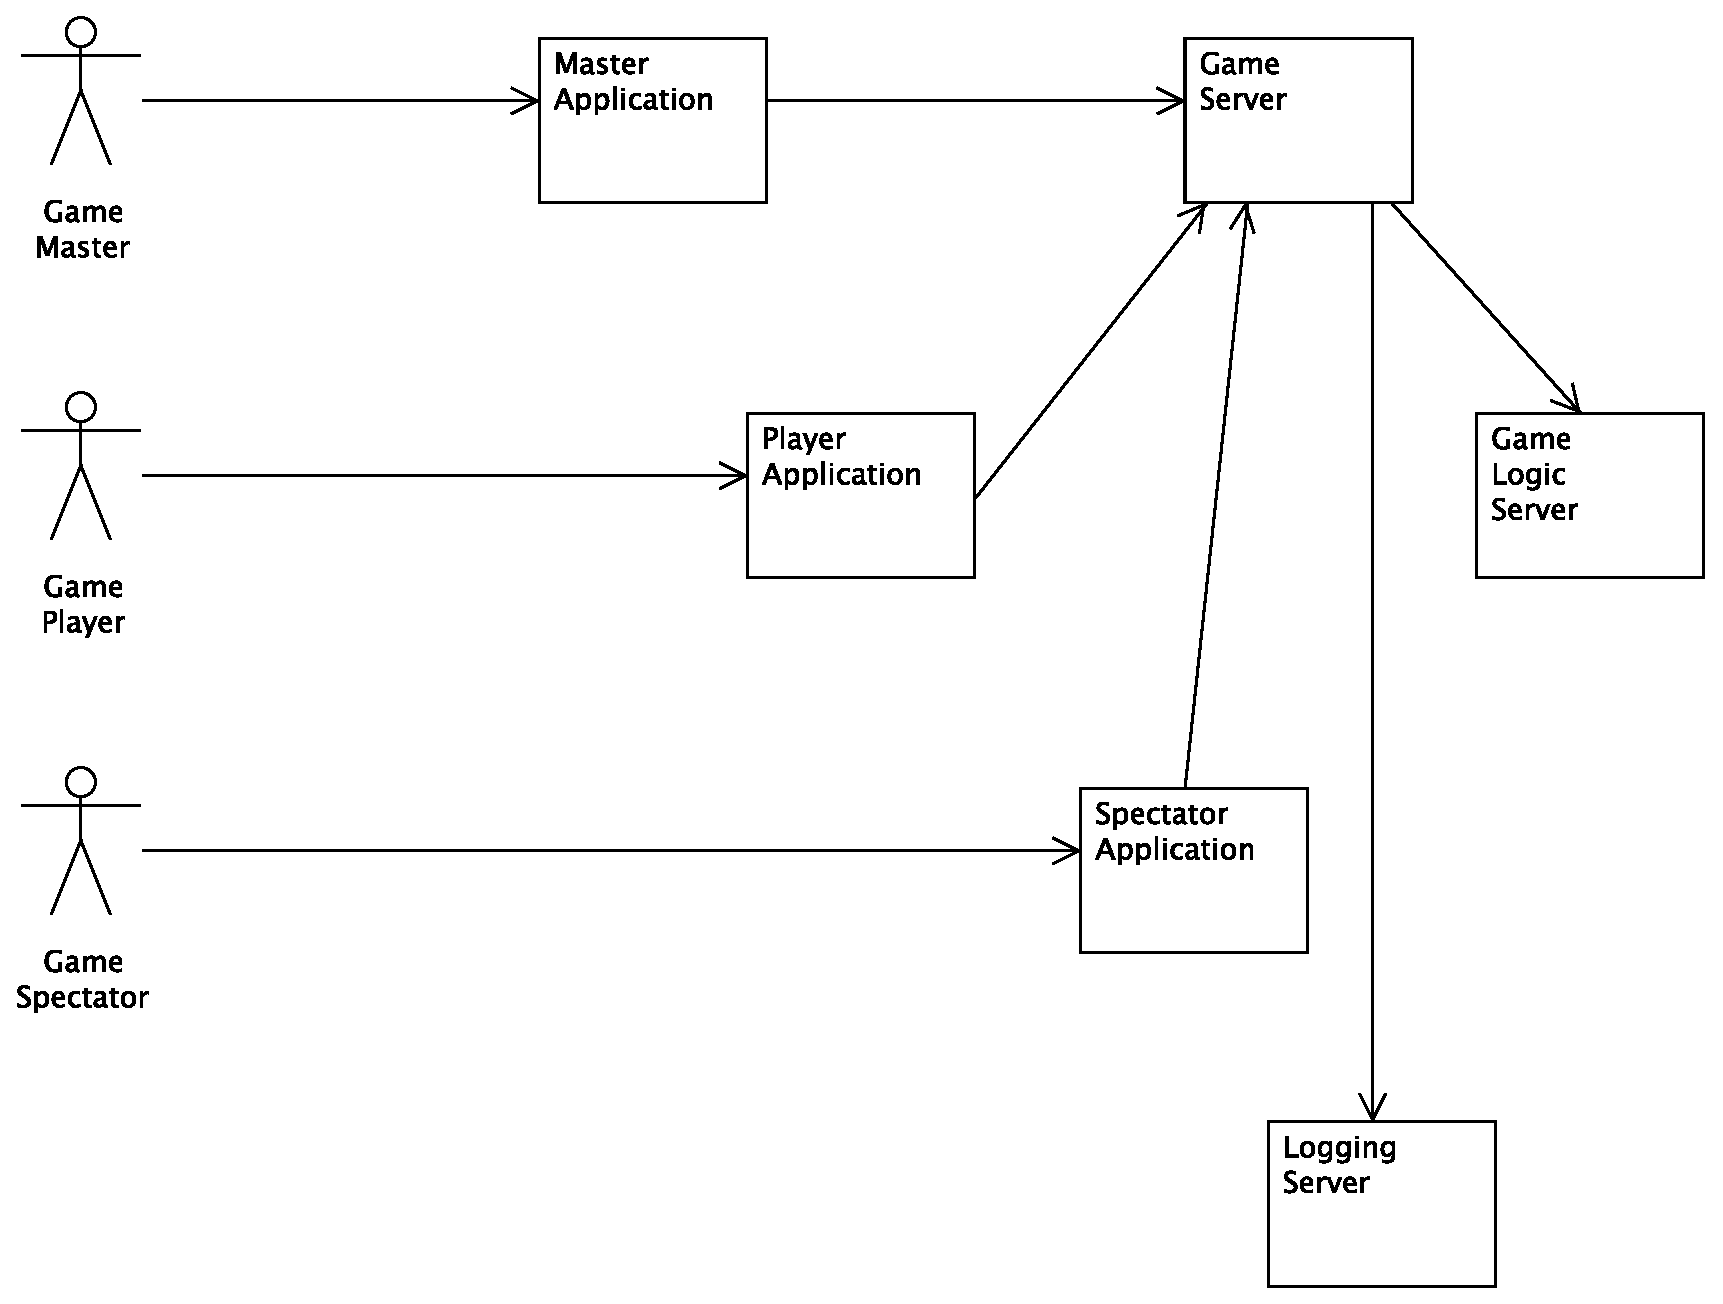
\includegraphics[scale=0.6]{Figures/_use_case_login}
\caption{Illustrative use case ---when log in using \textsf{XML-RPC}}
\label{F_use_case_login}
\end{center}
\end{figure}

\begin{figure}[htbp!]
\begin{center}
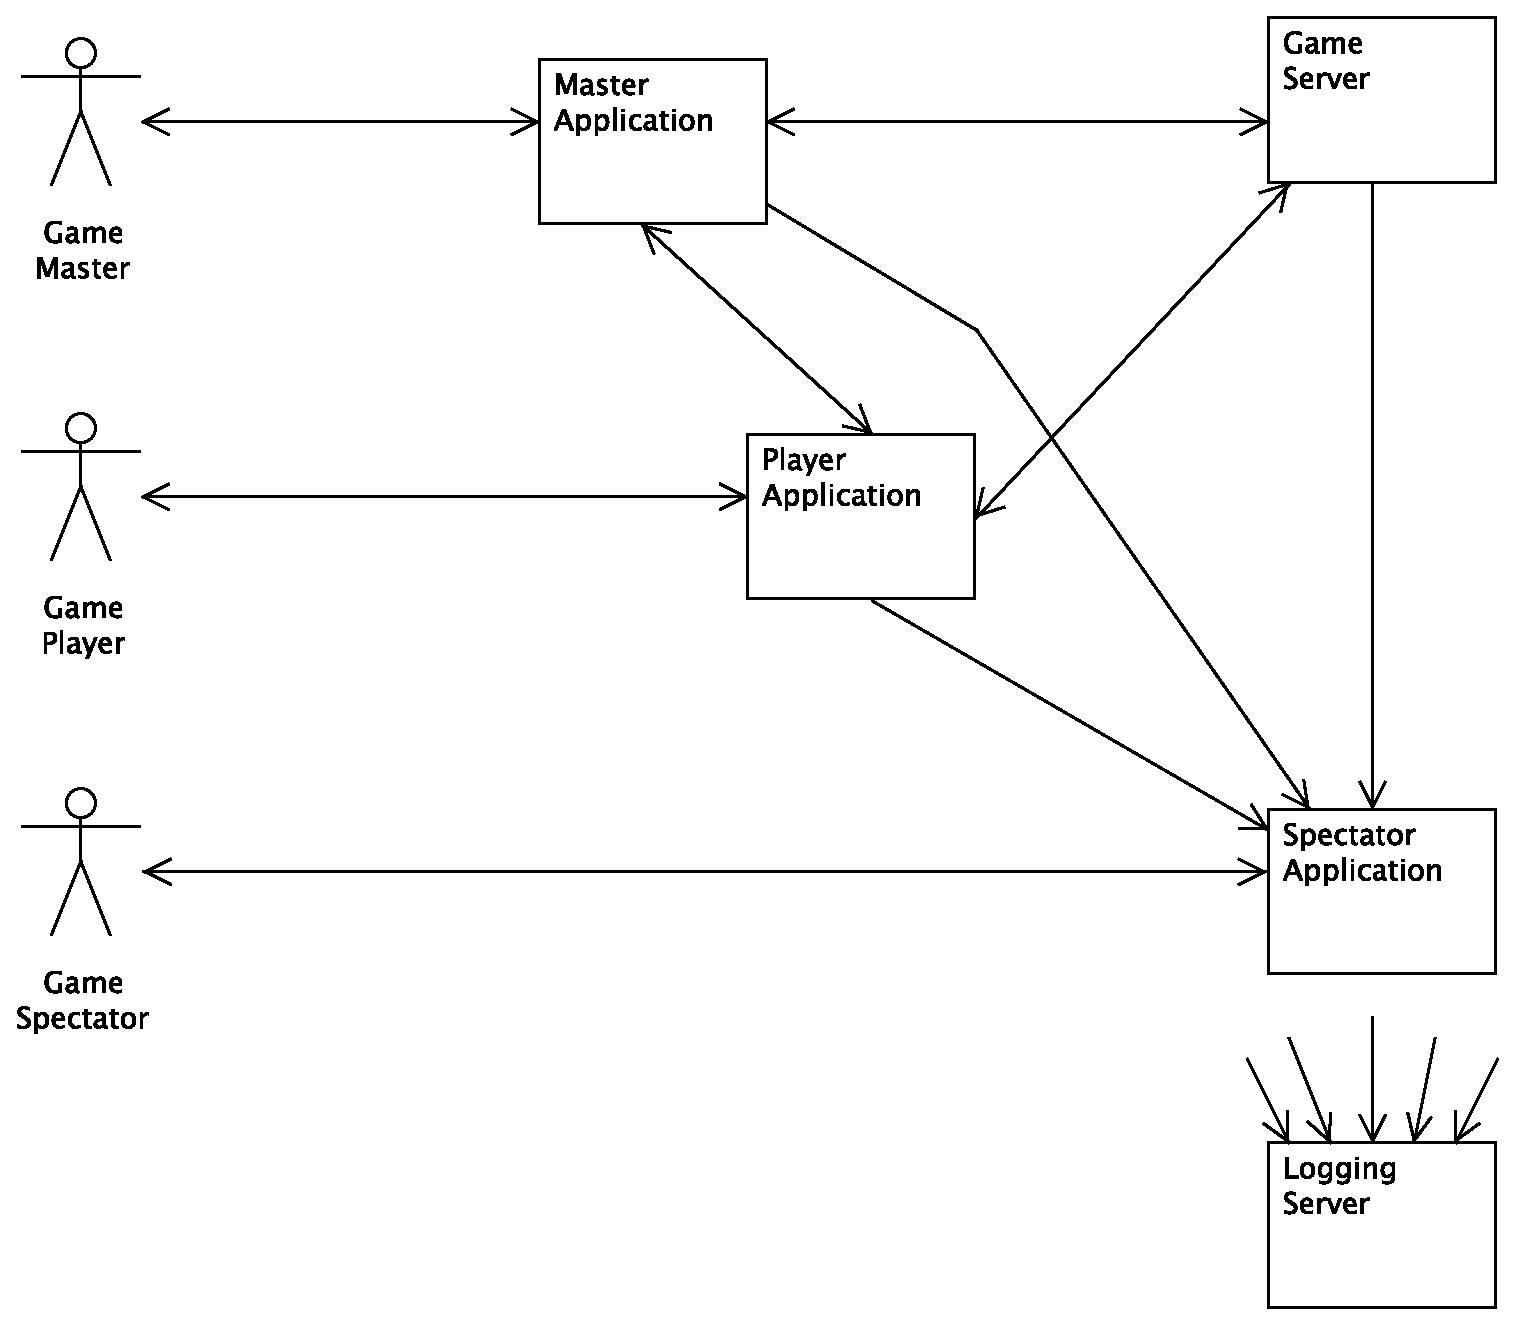
\includegraphics[scale=0.6]{Figures/_use_case}
\caption{Illustrative use case ---during the game play using\textsf{RabbitMQ}}
\label{F_use_case}
\end{center}
\end{figure}

% actors
% dessin use case avec la plate-forme TOTEM comme une bo�te noire et les acteurs
% - game platform admin
%   - Django
%   - RabbitMQ
% - game master
% - player
% - spectator

% illustrative scenario
% dessins activit�s du d�marrage d'un jeu
% - sc�nario de l'application exemple +
%   figure 4 (Activity diagram of the creation of the game and the
%             game instance, and of the joining of players and spectators)
%   - 1 couleur par acteur
%   - �v�nements, actions
%     - terminologie pour admin sys Django et RabbitMQ
